\documentclass[a4paper,12pt,oneside,openright]{report}

% ============================================================
% MATHÉMATIQUES (AVANT polyglossia/bidi)
% ============================================================
\usepackage{amsmath}
\usepackage{amssymb}

% ============================================================
% GRAPHIQUES & COULEURS
% ============================================================
\usepackage{graphicx}
\usepackage[table]{xcolor}
\definecolor{mycolor}{HTML}{1A4BC7}
\definecolor{quotemark}{gray}{0.7}
\definecolor{bleuPrev}{RGB}{52, 120, 190}
\definecolor{roseReel}{RGB}{210, 90, 120}
\graphicspath{{../images/}}
\definecolor{MYCOLOR}{RGB}{0,102,204}

% ============================================================
% MISE EN PAGE
% ============================================================
\usepackage[a4paper,width=150mm,top=20mm,bottom=25mm,bindingoffset=5mm]{geometry}
\usepackage{pdflscape}
\usepackage{fancyhdr}
\setlength{\headheight}{15pt}
\usepackage{ragged2e}
\usepackage{titlesec}
\usepackage{titletoc}
\usepackage{marginnote}
\usepackage{afterpage}
\usepackage{forest}

% ============================================================
% POLICES — XeLaTeX
% ============================================================
\usepackage{fontspec}
\usepackage{lettrine}

% ============================================================
% TABLEAUX
% ============================================================
\usepackage{booktabs}
\usepackage{array}
\usepackage{longtable}
\usepackage{multirow}
\usepackage{makecell}
\usepackage{tabularx}
\usepackage{tabularray}
\usepackage{rotating}

% ============================================================
% FIGURES
% ============================================================
\usepackage{float}
\usepackage{wrapfig}
\usepackage{subfigure}
\usepackage[rightcaption]{sidecap}
\usepackage{pdfpages}
\usepackage{adjustbox}

% ============================================================
% DIAGRAMMES
% ============================================================
\usepackage{tikz}
\usepackage{pgfgantt}

% ============================================================
% LISTES & DIVERS
% ============================================================
\usepackage{enumitem}
\usepackage{comment}
\usepackage{listings}
\lstdefinelanguage{json}{
  basicstyle=\ttfamily\small,
  showstringspaces=false,
  breaklines=true,
  morestring=[b]",
  stringstyle=\color{blue},
  literate=
   *{0}{{{0}}}{1}
    {1}{{{1}}}{1}
    {2}{{{2}}}{1}
    {3}{{{3}}}{1}
    {4}{{{4}}}{1}
    {5}{{{5}}}{1}
    {6}{{{6}}}{1}
    {7}{{{7}}}{1}
    {8}{{{8}}}{1}
    {9}{{{9}}}{1}
    {:}{{{\color{black}{:}}}}{1}
    {,}{{{\color{black}{,}}}}{1}
    {\{}{{{\color{black}{\{}}}}{1}
    {\}}{{{\color{black}{\}}}}}{1}
    {[}{{{\color{black}{[}}}}{1}
    {]}{{{\color{black}{]}}}}{1},
}
\usepackage{appendix}
\usepackage{pifont}
\usepackage[nottoc]{tocbibind}
\usepackage{tcolorbox}
\usepackage{glossaries}

% ============================================================
% BIBLIOGRAPHIE
% ============================================================
\usepackage{cite}

% ============================================================
% HYPERLIENS
% ============================================================
\usepackage[hypertexnames=false,bookmarks=false]{hyperref}
\usepackage{url}
\hypersetup{
  colorlinks=true,
  linkcolor=black,
  citecolor=black,
  filecolor=black,
  urlcolor=black
}

% ============================================================
% LANGUES — après les packages techniques (compatibilité bidi)
% ============================================================
\usepackage{polyglossia}
\setmainlanguage{english}
\setotherlanguage{arabic}
\IfFontExistsTF{XCharter}{%
  \setmainfont{XCharter}
}{%
  \setmainfont{DejaVu Serif}
}
\IfFontExistsTF{Traditional Arabic}{%
  \newfontfamily\arabicfont[Script=Arabic]{Traditional Arabic}
}{%
  \IfFontExistsTF{Amiri}{%
    \newfontfamily\arabicfont[Script=Arabic]{Amiri}
  }{%
    \newfontfamily\arabicfont[Script=Arabic]{Arial}
  }
}

% ============================================================
% COMPTEURS
% ============================================================
\setcounter{tocdepth}{4}
\setcounter{secnumdepth}{4}

% ============================================================
% EN-TÊTES & PIEDS DE PAGE
% ============================================================
\pagestyle{fancy}
\renewcommand{\headrulewidth}{0pt}
\renewcommand{\footrulewidth}{0.4pt}
\rhead{\thepage}

% ============================================================
% FORMAT DES CHAPITRES
% ============================================================
\titleformat{\chapter}[display]
  {\normalfont\Large\raggedleft}
  {\MakeUppercase{\chaptertitlename}%
  \rlap{ \resizebox{!}{1.5cm}{\thechapter} \rule{5cm}{1.5cm}}}
  {10pt}{\Huge}
\titlespacing*{\chapter}{0pt}{30pt}{20pt}

% ============================================================
% ENVIRONNEMENT FQUOTE (citation stylisée)
% ============================================================
\makeatletter
\def\fquote{%
    \@ifnextchar[{\fquote@i}{\fquote@i[]}%]
}%
\def\fquote@i[#1]{%
    \def\tempa{#1}%
    \@ifnextchar[{\fquote@ii}{\fquote@ii[]}%]
}%
\def\fquote@ii[#1]{%
    \def\tempb{#1}%
    \@ifnextchar[{\fquote@iii}{\fquote@iii[]}%]
}%
\def\fquote@iii[#1]{%
    \def\tempc{#1}%
    \vspace{1em}%
    \noindent%
    \begin{list}{}{%
            \setlength{\leftmargin}{0.1\textwidth}%
            \setlength{\rightmargin}{0.1\textwidth}%
        }%
        \item[]%
        \begin{picture}(0,0)%
            \put(-15,-5){\makebox(0,0){\scalebox{3}{\textcolor{quotemark}{``}}}}%
        \end{picture}%
        \begingroup\itshape}%
\def\endfquote{%
    \endgroup\par%
    \makebox[0pt][l]{%
        \hspace{0.8\textwidth}%
        \begin{picture}(0,0)(0,0)%
            \put(15,15){\makebox(0,0){%
                    \scalebox{3}{\color{quotemark}''}}}%
        \end{picture}}%
    \ifx\tempa\empty%
    \else%
    \ifx\tempc\empty%
    \hfill\rule{100pt}{0.5pt}\\\mbox{}\hfill\tempa,\ \emph{\tempb}%
    \else%
    \hfill\rule{100pt}{0.5pt}\\\mbox{}\hfill\tempa,\ \emph{\tempb},\ \tempc%
    \fi\fi\par%
    \vspace{0.5em}%
\end{list}%
}%
\makeatother
\emergencystretch=3em
\hfuzz=1000pt
\vfuzz=1000pt
\hbadness=10000
\vbadness=10000
\makeatletter
\def\input@path{{main chapters/}{./}}
\makeatother

% ============================================================
% DOCUMENT
% ============================================================
\begin{document}
	\flushbottom
	\sloppy
	\hfuzz=\maxdimen
	\vfuzz=\maxdimen
	\hbadness=10000
	\vbadness=10000
	\emergencystretch=10em
	\tolerance=9999
	
	\pagenumbering{Roman}
	\graphicspath{{pictures/}}
	\newcommand{\HRule}{\rule{\linewidth}{0.5mm}}
	
	\newcommand{\cleartoodd}{\clearpage}
	
	\renewcommand{\headrulewidth}{2pt}
	\addtocontents{toc}{\vspace{2cm}}
	
	\begin{titlepage}
		\newgeometry{margin=0pt}
		\thispagestyle{empty}
		\noindent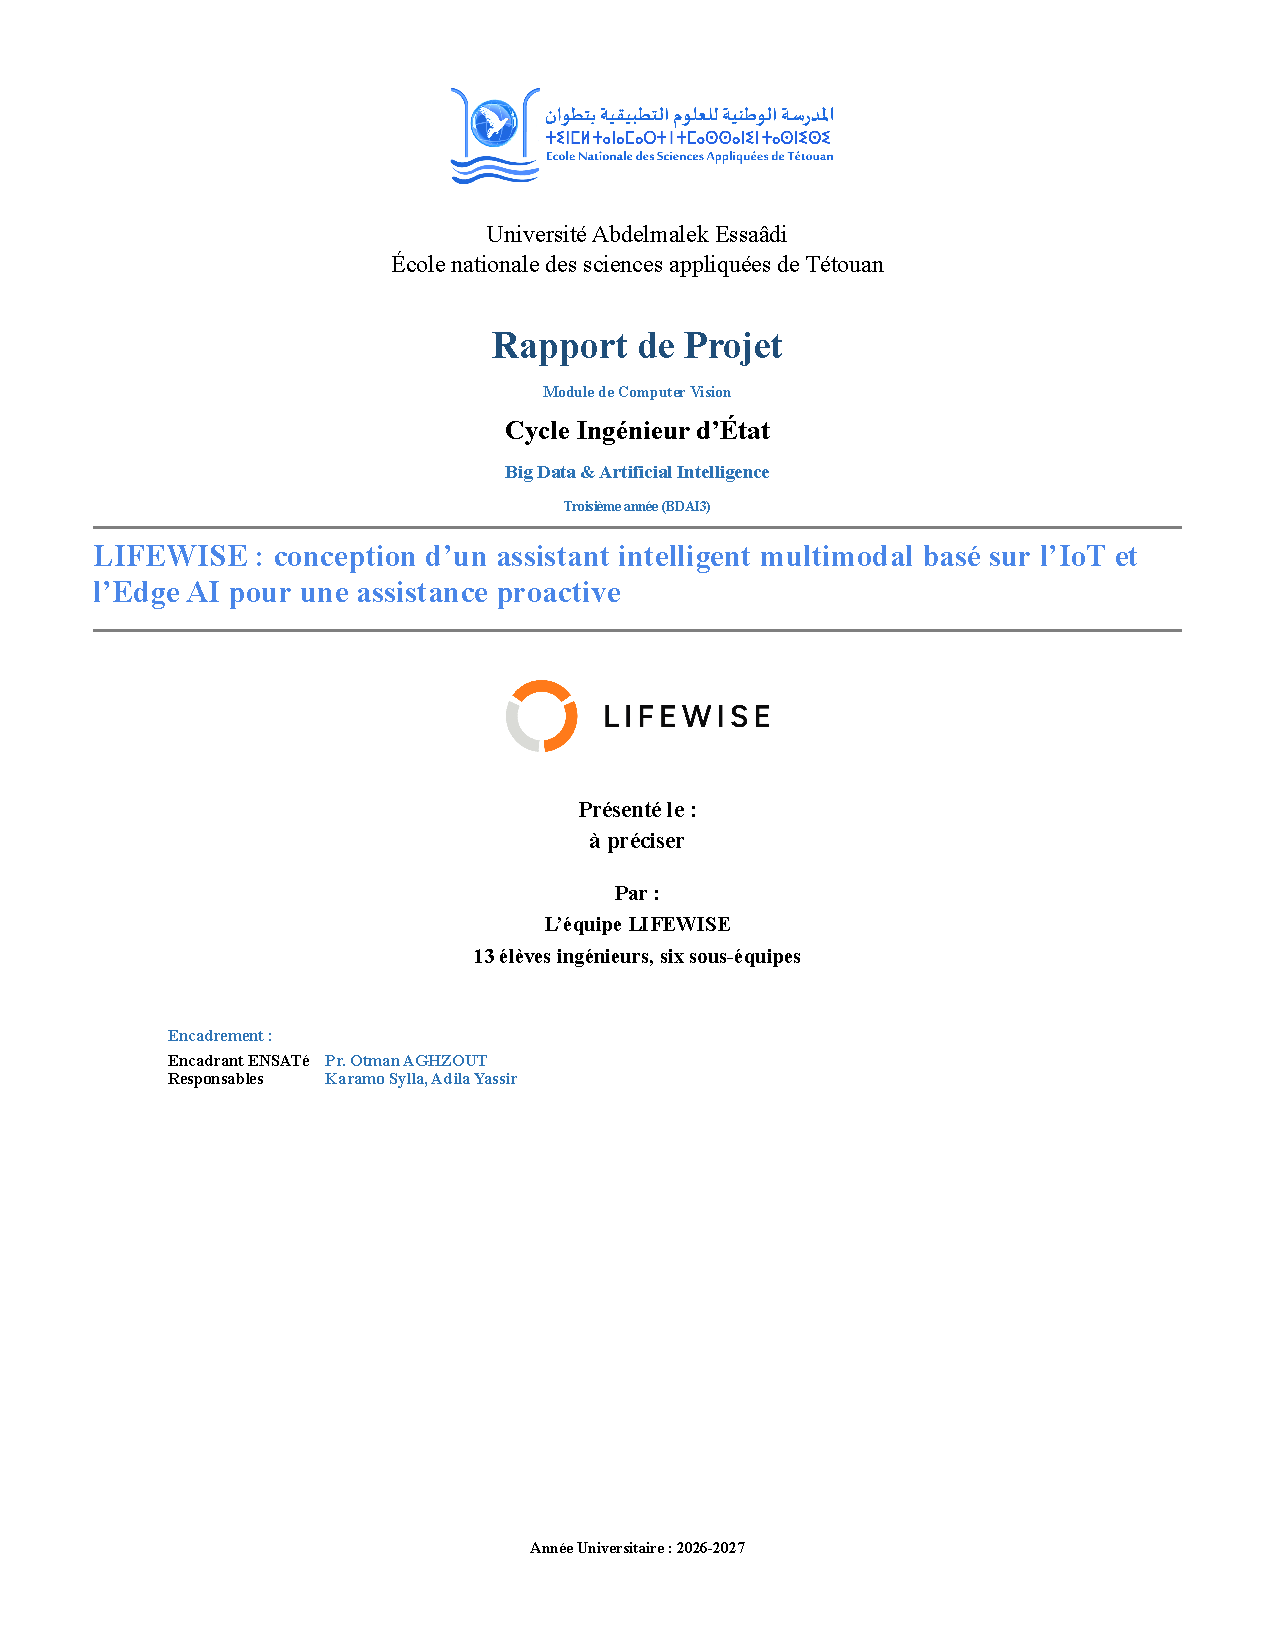
\includegraphics[page=1,width=\paperwidth,height=\dimexpr\paperheight-1pt\relax,keepaspectratio=false]{Figures/Cover/LIFEWISE_Page_de_garde.pdf}
		\restoregeometry
	\end{titlepage}
	\include{before}
	\include{02-Dedicaces}
	\include{03-Acknowledgment}
	\include{04-Resume}
	\chapter*{\textcolor{mycolor}{\textarabic{ملخص}}}
\addcontentsline{toc}{chapter}{\textarabic{ملخص}}

\begin{Arabic}
\large

تنتظر المساعدات الشخصية الحالية أن يطلب منها المستخدم شيئًا: طرح سؤال، أو برمجة تذكير، أو فتح تطبيق. غير أن اللحظة التي نحتاج فيها إلى المساعدة، كلحظة مغادرة المنزل، هي بالضبط اللحظة التي لا نفكر فيها في ذلك.

يقترح مشروع \textbf{LIFEWISE} مساعدًا سياقيًا يراقب الوضع ويتدخل من تلقاء نفسه. يجمع جهاز صغير مزوَّد بكاميرا وبمستشعرات للحركة وللباب وللإضاءة مؤشرات عن المحيط. يصف نموذج خفيف للرؤية واللغة \textbf{(VLM)} ما تراه الكاميرا، ثم يقارن نموذج لغوي صغير \textbf{(SLM)}، تسبقه قواعد مكتوبة، هذا الوصف بالسياق (المواعيد والعادات) ويقرر ما إذا كان ينبغي تنبيه المستخدم على هاتفه. تُحفظ الأحداث في قاعدة بيانات محلية \textbf{SQLite} ويمكن الاطلاع عليها عبر لوحة قيادة على الويب. وتبقى جميع المعالجات محلية، على جهاز \textenglish{\textbf{Raspberry Pi}} يُستعمل منصةً لتجربة الذكاء الاصطناعي على الحافة.

يستهدف النموذج الأولي سيناريو تجريبيًا: المساعدة عند مغادرة المنزل. عند لحظة الخروج، يتحقق النظام من أن الهاتف والمفاتيح والمحفظة مأخوذة، وإذا لم يظهر أحدها يدعو المستخدم إلى التحقق منه. يبقى التنبيه دعوةً إلى التحقق، لأن الكاميرا لا تثبت إلا أن الشيء غير موجود في مجال رؤيتها، ولا تثبت أبدًا أنه نُسي.

ينجز المشروع ثلاثة عشر طالبًا مهندسًا موزعين على ست فرق فرعية، لكل حلقة من السلسلة فريق. ويعرض هذا التقرير سياق المشروع، والدراسة النظرية، والتصميم، والإنجاز، والتقييم.

\vspace{0.5cm}

\textbf{الكلمات المفتاحية}: الرؤية الحاسوبية، الذكاء الاصطناعي على الحافة، إنترنت الأشياء، نموذج الرؤية واللغة، النموذج اللغوي الصغير، المساعدة الاستباقية.

\end{Arabic}

	\include{05-Abstract}
	\include{06-Content_Table}
	\include{07-Abbreviation}
	\include{08-Figures_List}
	\pagenumbering{arabic}
	\setcounter{page}{1}
	\include{09-General Introduction}
	
	\cleartoodd
	\include{Chapter 1}
	%
	\cleartoodd
	\include{Chapter 2}
	%
	\cleartoodd
	\include{Chapter 3}
	%
	\cleartoodd
	\include{Chapter4_fixed}
	%
	\cleartoodd
	\include{Chapter5}
	%
	\include{General conclusion}
	\include{GFuture Works}
	%
	\cleartoodd
	\begingroup
\titleformat{\chapter}[display]
  {\normalfont\Large\raggedright}
  {\MakeUppercase{\chaptertitlename}%
  \rlap{ \resizebox{!}{1.5cm}{\thechapter} \rule{5cm}{1.5cm}}}
  {10pt}{\Huge}
\chapter*{\textcolor{mycolor}{Webographie}}
\endgroup
\addcontentsline{toc}{chapter}{Webographie}
\fancyhf{} % Clear header and footer
\fancyhead{} % Clear header

\section*{Modèles d'intelligence artificielle}

\begin{enumerate}
\setcounter{enumi}{0}

\item Liu, H., Li, C., Wu, Q., Lee, Y. J. (2023).
\textit{Visual Instruction Tuning}. Advances in Neural Information Processing Systems (NeurIPS).\\
\url{https://arxiv.org/abs/2304.08485}

\item Moondream2, modèle vision-langage compact.\\
\url{https://huggingface.co/vikhyatk/moondream2}\\
\textit{Consulté le : Novembre 2026}

\item Redmon, J., Divvala, S., Girshick, R., Farhadi, A. (2016).
\textit{You Only Look Once: Unified, Real-Time Object Detection}. CVPR.\\
\url{https://arxiv.org/abs/1506.02640}

\item Abdin, M. et al. (2024).
\textit{Phi-3 Technical Report: A Highly Capable Language Model Locally on Your Phone}.\\
\url{https://arxiv.org/abs/2404.14219}

\item Yang, A. et al. (2024). \textit{Qwen2 Technical Report}.\\
\url{https://arxiv.org/abs/2407.10671}

\item Jiang, A. Q. et al. (2023). \textit{Mistral 7B}.\\
\url{https://arxiv.org/abs/2310.06825}

\end{enumerate}

\section*{Outils et documentation}

\begin{enumerate}
\setcounter{enumi}{6}

\item OpenCV Documentation.\\
\url{https://docs.opencv.org/}\\
\textit{Consulté le : Novembre 2026}

\item PyTorch Documentation.\\
\url{https://pytorch.org/docs/}\\
\textit{Consulté le : Novembre 2026}

\item Hugging Face Transformers Documentation.\\
\url{https://huggingface.co/docs/transformers}\\
\textit{Consulté le : Novembre 2026}

\item Ollama, exécution locale de modèles de langage.\\
\url{https://ollama.com/}\\
\textit{Consulté le : Novembre 2026}

\item SQLite Documentation.\\
\url{https://www.sqlite.org/docs.html}\\
\textit{Consulté le : Novembre 2026}

\item Raspberry Pi Documentation.\\
\url{https://www.raspberrypi.com/documentation/}\\
\textit{Consulté le : Novembre 2026}

\end{enumerate}

\noindent\textit{Chaque sous-équipe complète cette liste avec les références qu'elle cite.}

	%
	\cleartoodd
	\include{Annexe A}
	
\end{document}